\section{Граничное управление нелинейными волнами деформации в слое двухатомного кристалла}
\begin{frame}[plain, noframenumbering]
    \begin{center}
        \Large
        Граничное управление нелинейными волнами деформации в слое двухатомного кристалла
    \end{center}
\end{frame}

\subsection{Уравнения модели}

\begin{frame}
	\frametitle{Постановка задачи}
Рассматривается изотропный упругий слой,
\begin{itemize}
	\item неограниченной длины в горизонтальном направлении $x$;
	\item шириной $2 H$ в вертикальном направлении $y$;
	\item нижняя поверхность слоя соответствует $y = -H$, верхняя --- $y = H$;
	\item двухатомной структуры.
\end{itemize}   

Вид плотности потенциальной энергии определяется исходя из предположений о двухатомной структуре материала и характере взаимодействия между соседними частицами.

\end{frame}

\begin{frame}
	\begin{center}
		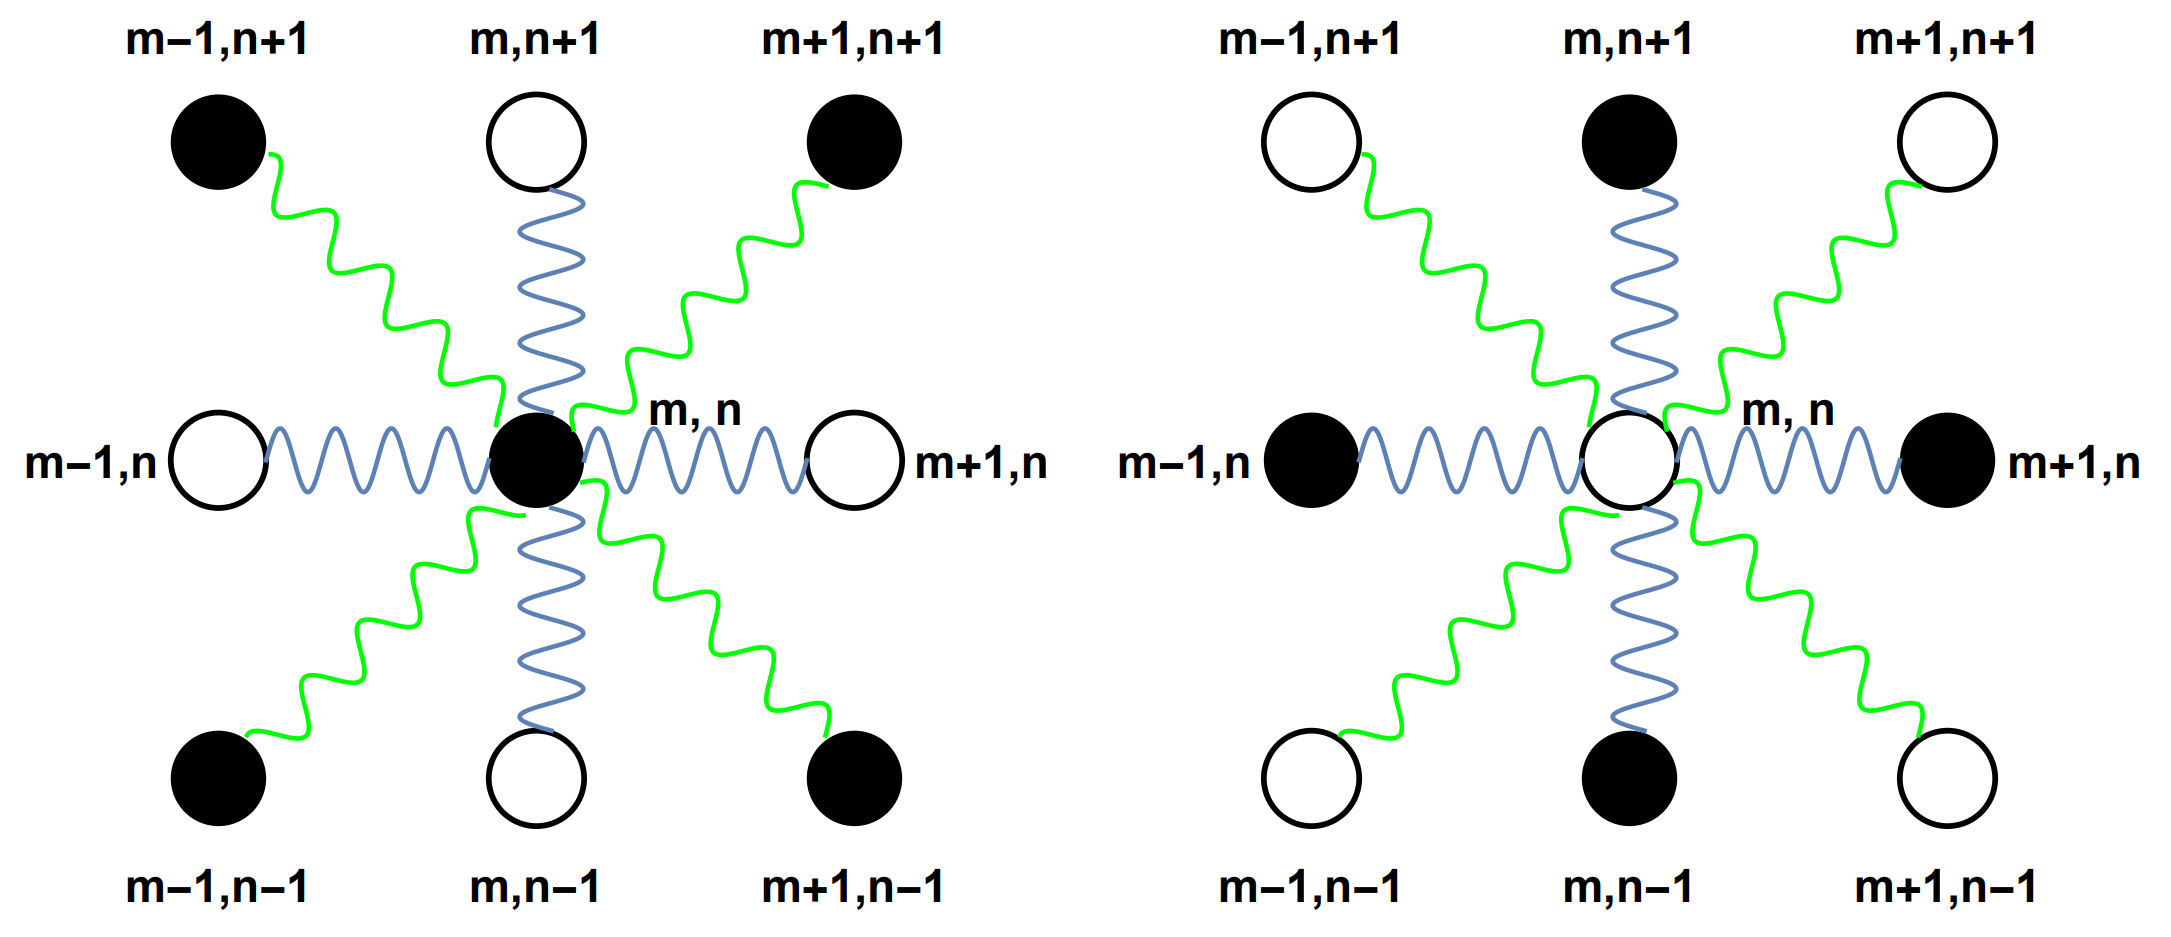
\includegraphics[width=0.85\linewidth]{lattice.png}
	\end{center}
	Система описывается функциями $U$, $u$, $V$, $v$,
	
	$$
	U~=~\frac{m_1~u_1+m_2~u_2}{m_1+m_2},~V=\frac{m_1~v_1+m_2~v_2}{m_1+m_2},
	$$
	$$
	u=\frac{u_1-u_2}{h},~v=\frac{v_1-v_2}{h},
	$$
	где $u_i$, $v_i$ --- горизонтальные и вертикальные смещения элементов двухатомной решетки с массой $m_i$ в континуальном приближении при $h \ll 1$, $i=1,2$ \footnotemark.

\footnotetext[1]{Two-Dimensional Modeling of Diatomic Lattice / A. V. Porubov // Advanced Structured Materials. — Springer International Publishing, 2018. -- С. 263—272.}	
\end{frame}


\begin{frame}
Уравнения движения выводятся с использованием принципа Гамильтона-Остроградского,

$$
\delta \left( \int_{t_0}^{t_1}dt \int_{-H}^{H} dy \int_{-\infty}^{\infty}\left( K - \Pi \right)  \:   dx \right)+ \delta A_1 + \delta A_2=0.
$$

Плотность кинетической энергии равна
$$
	K = \frac{1}{2} \rho (U_t^2 + V_t^2) + \frac{1}{2} \eta (u_t^2 + v_t^2),
$$
\begin{small}
$$
\rho = \frac{m_1+m_2}{h^3}, \quad \eta = \frac{m_1 m_2}{(m_1 + m_2)h}.
$$
\end{small}

Плотность потенциальной энергии условно разделена на две составляющих,
$$
\Pi = \Pi_l + \Pi_{nl}.
$$

\end{frame}


\begin{frame}
	
Линейная часть потенциальной энергии,
\begin{small}
$$
\Pi_l = \frac{C_1}{h} \left(u^2 + v^2\right) + \frac{C_1+C_2}{h}\left(U_x^2+V_y^2\right) +\frac{C_2}{h}\left(U_y^2 + V_x^2 + 2U_x V_y + 2 U_y V_x\right) +
$$
$$
\frac{h\left(C_2\left(m_1^2 + m_2^2\right) - 2C_1 m_1 m_2\right)}{2\left(m_1^2 + m_2^2\right)}\left(u_x^2 + v_y^2\right) + \frac{\left(m_2-m_1\right)\left(C_1+C_2\right)}{m_1+m_2}\left(u_x U_x + v_y V_y\right) +
$$
$$
\frac{C_2 h\left(m_1^2+m_2^2\right)}{2\left(m_1+m_2\right)^2}\left(u_y^2+v_x^2+2u_y v_x + 2u_x v_y\right) +
$$
$$
\frac{C_2\left(m_2 - m_1\right)}{m_1 + m_2}\left(u_y U_y+v_x V_x + u_y V_x + u_x V_y + v_y U_x + v_x U_y\right)
$$
\end{small}

Нелинейная часть потенциальной энергии\footnotemark,
\begin{small}
$$
\Pi_{nl} = \left( p - s_{xx} U_x - s_{yx} \left( U_y + V_x\right) - s_{yy} V_y\right) \left( 1- \cos{(u+v)}\right) \label{pot}
$$
\end{small}		
\footnotetext[2]{The solutions of equations for nonlinear model of deformation of the crystal media allowing martensitic transformations / E. L. Aero, A. N. Bulygin, Y. V. Pavlov // 2017 Days on Diffraction (DD). -- IEEE, 06.2017.
}
\end{frame}

\begin{frame}
\frametitle{Граничные условия}
	
	Выражение для напряжений на границе слоя при $y=-H$ соответствует модели Керра\footnotemark, $q_1$, $q_2$ --- константы, $k_d ~> ~0$ --- коэффициент трения по закону Амонтона-Кулона,
	$$
		\sigma_{y}=q_1 V + q_2 V_t , ~
		\tau_{xy}= k_d (q_1 V + q_2 V_t) \quad | \quad y = -H
	$$
	На верхнюю границу при $y=H$ действует распределенная нагрузка произвольного вида,
	$$
		\sigma_{y}=f_{N}, ~\tau_{xy}=f_{\tau} \quad | \quad y = H
	$$
	
	Соответствующие элементарные работы,
	\begin{small}
	$$
		\delta A_1 =  \int_{t_0}^{t_1} dt\int_{-\infty}^{\infty}f_{N}\delta V \:  dx +\int_{t_0}^{t_1} dt  
		\int_{-\infty}^{\infty} f_{\tau}\delta U \: dx ,
	$$
	$$s
		\delta A_2 =  \int_{t_0}^{t_1} dt \int_{-\infty}^{\infty}(q1_1 V + q_2 V_t)\delta V \:  dx + \int_{t_0}^{t_1} dt
		\int_{-\infty}^{\infty}k_d(q_1 V + q_2 V_t)\delta U \:  dx. 
	$$
	\end{small}

\footnotetext[3]{Elastic and Viscoelastic Foundation Models / A. D. Kerr // Journal of Applied Mechanics. -- 1964. -- Сент. -- Т. 31, № 3. -- С. 491-498.}
\end{frame}

\begin{frame}
\frametitle{Уравнения движения для продольных волн}
\begin{small}	
	Система уравнений движения, полученная из вариационного принципа не приведена в силу громоздкости получаемых выражений и требует применения некоторых упрощений.
	
\begin{itemize}
	\item { Рассматриваются продольные волны, решения в виде степенного ряда по $y$
		\small{
		$$
			U=U_0(x,t)+B_1(x,t)~y+B_2(x,t)~y^2,~u=u_0(x,t)+b_1(x,t)~y+b_2(x,t)~y^2, \label{Usol}
		$$
		$$
			V=y~A(x,t), v=y~a(x,t). \label{Vsol}
		$$
		}
	}
	\item {Упрощается вид нелинейности, предполагается
		$$
		s_{xx} \gg s_{yx}, s_{yy}
		$$
	}
\end{itemize}
	
	Одномерные уравнения для продольных волн относительно $U_0$, полученные в результате процедуры упрощения, имеют вид
\begin{small}
\begin{multline}
	\rho U_{0,tt}-F_1 U_{0,xx}-F_2 u_{0,xx}+F_{31} \left(\cos(u_0)\right)_x = F_5 f_\tau\\
	+ k_d q_1 \left(F_7 U_{0,x}+F_8 u_{0,x}\right)+k_d q_2 \left(F_{11} u_{0,xt}+ F_{13} U_{0,xt}\right),
\end{multline}
\begin{equation}
	\eta u_{0,tt}+f_1 u_0+f_2 u_{0,xx}+f_3 U_{0,xx}+\left(p-s_{xx} U_{0,x}\right)\sin(u_0)=0.  
\end{equation}

\end{small}
\end{small}
\end{frame}

\begin{frame}
	Дальнейшие упрощения связаны с
	\begin{itemize} 
		\item рассмотрением слабонелинейного случая, $u_0 \ll 1$, $U_{0, x} \ll 1$, система приводится к виду
	\begin{multline}
		\rho U_{0,tt}- F_1 U_{0,xx}- F_2 u_{0,xx}-F_{31} u_0 u_{0,x}=F_5 f_\tau\\
		+k_d q_1 (F_7 U_{0,x}+F_8 u_{0,x})+ k_d q_2 (F_{11} u_{0,xt}+ F_{13} U_{0,xt}),
	\end{multline}
	\begin{equation}
		(f_1+p)u_0+f_3 U_{0,xx}-s_{xx} u_0 U_{0,x}=0.
	\end{equation}
		\item рассмотрением длинных волн ($U_{0, xx} \ll U_{0, x}$) и использованием принципа асимптотического подчинения для функции $u$, система сводится к уравнению относительно $U_0$,
		\begin{small}
		\begin{multline}
		\rho U_{0,tt}- F_1 U_{0,xx}+ \frac{f_3 F_2}{f_1+p}U_{0,xxxx}\\+\frac{f_3 s_{xx} F_{2}}{2(f_1+p)^2} (U_{0,x}^2)_{xxx}
		-\frac{f_3^2 F_{31}}{2(f_1+p)^2} (U_{0,xx}^2)_{x}=\\
			F_5 f_\tau+k_d q_1 F_7 U_{0,x} + k_d q_2 F_{11}U _{0,xt}
		\end{multline}
		\end{small}
	\end{itemize}

\end{frame}


\subsection{Алгоритм управления}

\begin{frame}
\frametitle{Алгоритм управления}

Несколько слов о разработанном в предшествующих работах алгоритме управления. В качестве примера рассматривается локализация волновых решений модифицированного уравнения синус-Гордона,
$$
	U_{tt}-U_{xx}+\sin(U)+\omega(x,t)=0,
$$
где $\omega$ --- функция распределенного управления с обратной связью, выражаемая следующим образом,
$$
\omega(x,t)=\gamma \left(\alpha e(x,t)+\alpha_1 e_t(x,t)\right),
$$
$$
e(x,t)=U(x,t)-U^*(x,t),
$$
$$
e_t(x,t)=U_t(x,t)-U^*_t(x,t).
$$
$U^*(x,t)$ --- целевая функция, в качестве которой можно выбрать колоколоообразный солитон, не являющийся точным решением УсГ.
\end{frame}

\begin{frame}
	\begin{figure}
		\begin{center}
			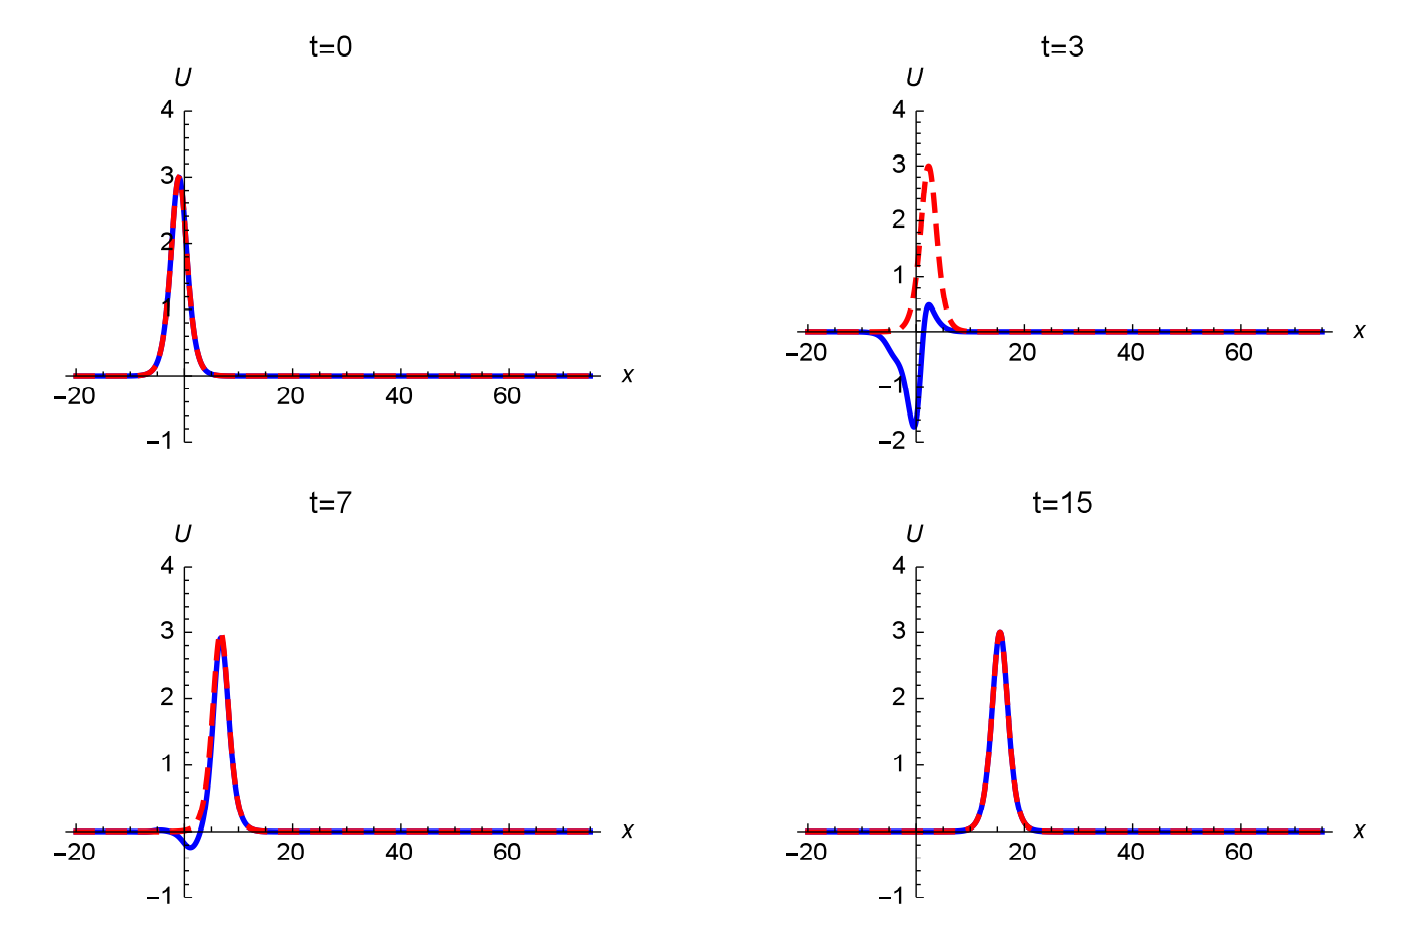
\includegraphics[width=0.9\textwidth]{control_example.png}
		\end{center}
		Пример работы алгоритма, включение при $t = 5$. Синяя линяя --- численное решение, красная пунктирная --- целевая функция вида $A~ {\text{sech}}^2(k (x- t+1))$.
	\end{figure}
\end{frame}

\begin{frame}
	\frametitle{Управление волнами деформации в слое}

Уравнение рассматриваемой системы,
\begin{multline*}
	\rho U_{0,tt}- F_1 U_{0,xx}+ \frac{f_3 F_2}{f_1+p}U_{0,xxxx}\\+\frac{f_3 s_{xx} F_{2}}{2(f_1+p)^2} (U_{0,x}^2)_{xxx}
	-\frac{f_3^2 F_{31}}{2(f_1+p)^2} (U_{0,xx}^2)_{x}=\\
	F_5 f_\tau+k_d q_1 F_7 U_{0,x} + k_d q_2 F_{11}U _{0,xt},
\end{multline*}
в правой части содержит член, который аналогичным образом может играть роль управляющей функции с обратной связью схожего вида,
$$
\omega(x,t)=\gamma \left(\alpha e_x(x,t)+\alpha_1 e_{xt}(x,t)\right),
$$
при выборе внешней нагрузки
$$
f_\tau=-\frac{k_d}{F_5}\left(q_1 F_7 U^*_{0,x}(x,t)+  q_2 F_{11} U_{0,xt}^*(x,t)\right).
$$
\end{frame}	

\subsection{Основные результаты}
\frametitle{Результаты расчетов}
\begin{frame}
	\begin{figure}
		\begin{center}
			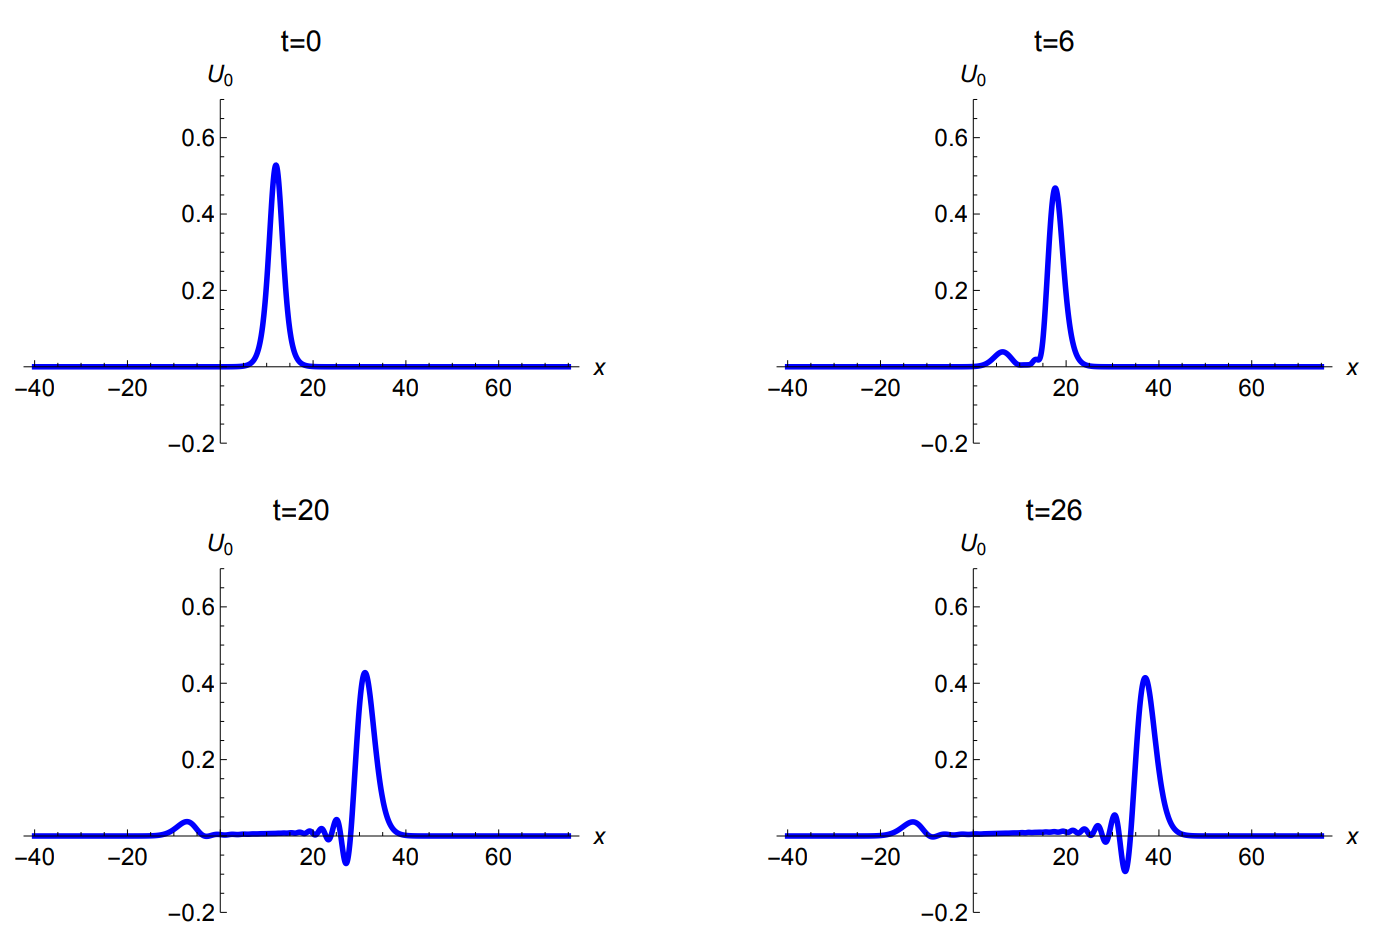
\includegraphics[width=0.9\textwidth]{fig_no_control.png}
		\end{center}
		Распространение колоколообразного начального возмущения вида $A~{\text{sech}}^2 (k (x-V t-x_0))$, внешняя нагрузка $f_\tau$ равна нулю.
	\end{figure}
\end{frame}

\begin{frame}
	\frametitle{Результаты расчетов}
	\begin{figure}
		\begin{center}
			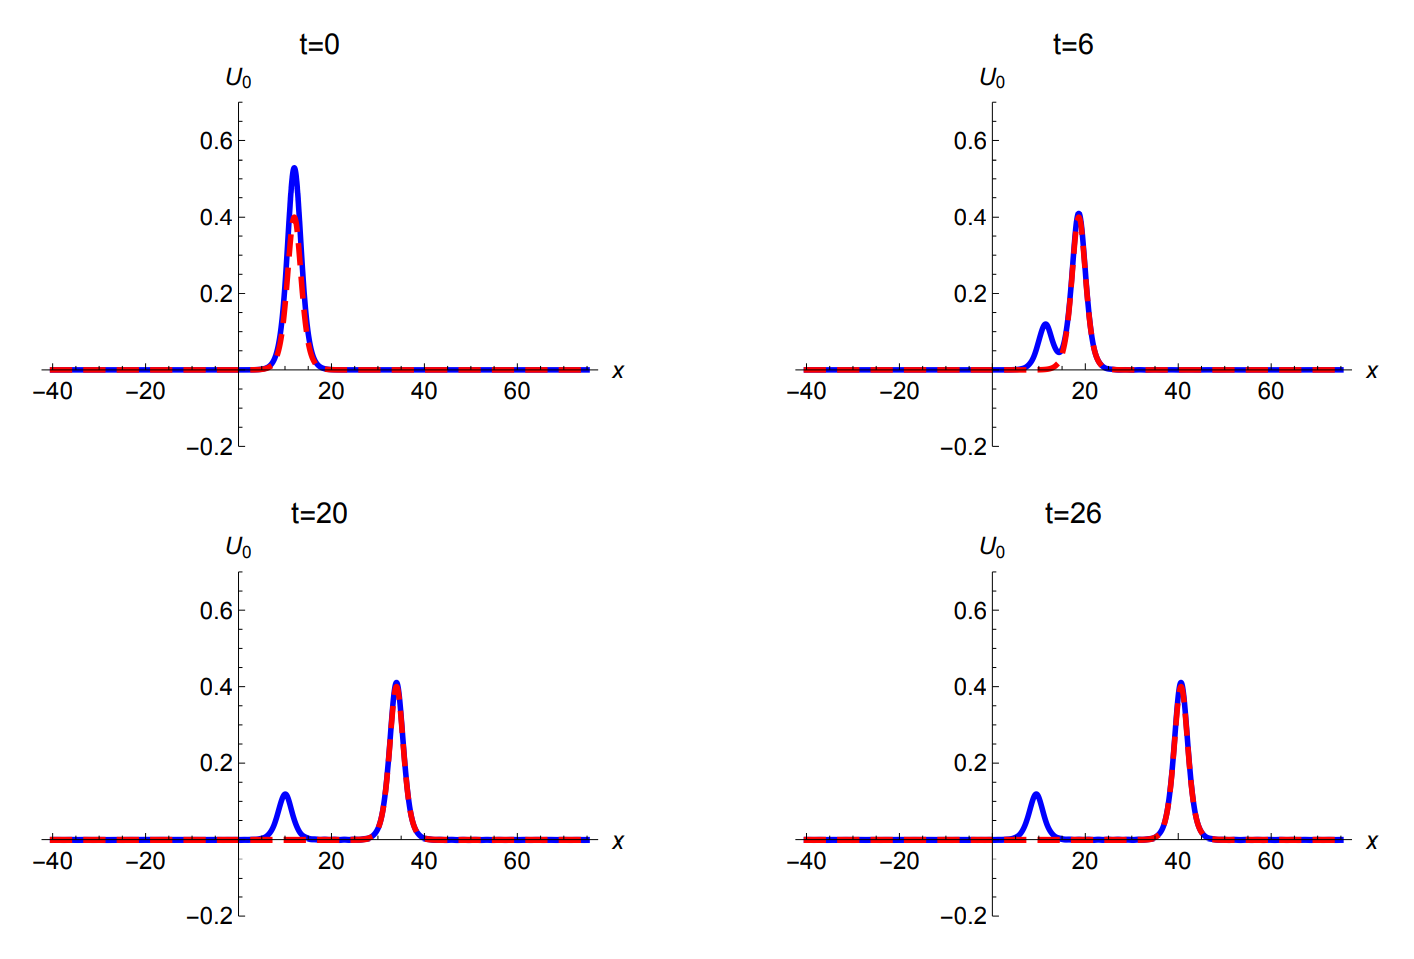
\includegraphics[width=0.9\textwidth]{fig_control.png}
		\end{center}
		Случай с внешней нагрузкой, обеспечивающей наличие управляющей $\omega$ в правой части уравнения. Целевая функция вида $A~{\text{sech}}^2 (k (x-V t-x_0))$.
	\end{figure}
\end{frame}

\begin{frame}
	\frametitle{Результаты}
	Основные результаты данной части работы заключаются в следующем,
	\begin{itemize}
		\item{Получены модельные уравнения, описывающие распространение нелинейных волн деформации в изотропном упругом слое заданной структуры;}
		\item{Показано, что модель допускает наличие распределенного управляющего воздействия с обратной связью, действующего на границе материала;}
		\item{Показано, что выбор нагрузки согласно алгоритму управления, разработанному ранее для схожих механических систем, обеспечивает возможность локализации волн в рассматриваемой системе. }
	\end{itemize}
\end{frame}

\section{Управление гармоническими волнами в акустическом метаматериале}
\begin{frame}[plain, noframenumbering]
	\begin{center}
		\Large
		Управление гармоническими волнами в акустическом метаматериале
	\end{center}
\end{frame}
\subsection{Уравнения модели}

\begin{frame}
	\frametitle{Постановка задачи}
	Рассматривается модель акустического метаматериала <<масса в массе>>, 
	\begin{itemize}
		\item одномерная цепочка, массы $m$ соединены упругими пружинами жесткости $\beta_0 m$;
		\item к каждой частице массы $m$ присоединена масса $m_1$ пружиной линейной жесткости $\beta_1 m_1$, $\eta = m_1/m$;
		\item массы $m_1$ между собой явно не взаимодействуют;
		\item расстояние между соседними частицами --- $h$.
	\end{itemize}   
	
	\begin{center}
		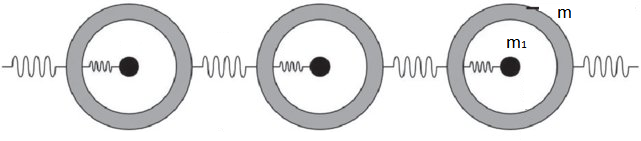
\includegraphics[width=0.7\textwidth]{mim.png}
	\end{center}
	
\end{frame}

\begin{frame}
	Уравнения движения в смещениях $x_n$, $y_n$ для масс $m$, $m_1$ соответственно, выражаются следующим образом,
\begin{equation}
	\ddot{x_n}=\beta_0 (x_{n-1}-2x_n+x_{n+1})+\eta \beta_1 (y_n-x_n), 
	\label{eq1}
\end{equation}
\begin{equation}
	\ddot{y_n}=-\beta_1 (y_n-x_n).
\end{equation}

В континуальном пределе, оставляя первый ненулевой член в ряде Тейлора, уравнения принимают вид
\begin{equation}
	u_{tt}=\beta_0 h^2 u_{xx}+\eta \beta_1 (v-u), \label{eq3}
\end{equation}
\begin{equation}
	v_{tt}=-\beta_1 (v-u). \label{eq4}
\end{equation}
	
\end{frame}

\begin{frame}
	Решения в виде бегущих волн
	$$
	u=A \exp (\imath(p~ x - \omega~ t- p~ x_0)), ~
	v=B \exp (\imath(p~ x - \omega~ t-p~ x_0)).
	$$
	Подстановка в уравнения модели дает
	$$
	A = \frac{\beta_1-\omega^2}{\beta_1}~B
	$$
	Дисперсионное соотношение
	$$
	\omega^4 -(\beta_1(1+\eta)+\beta_0 p^2 h^2)\omega^2+\beta_0 \beta_1 p^2 h^2=0.
	$$
	\begin{small}
	$$
		\omega_a^2=\frac{\beta_1(1+\eta)+\beta_0 h^2 p^2}{2}-\frac{\sqrt{D}}{2},
	$$
	$$
		\omega_o^2=\frac{\beta_1(1+\eta)+\beta_0 h^2 p^2}{2}+\frac{\sqrt{D}}{2},
	$$

	$$
	D=(\beta_1(1+\eta)+\beta_0 h^2 p^2)^2-4\beta_0 h^2 p^2.
	$$
	\end{small}
\end{frame}

\begin{frame}
	\begin{itemize}
		\item Акустическая ветвь лежит в диапазоне частот от $ 0 $ до $ \sqrt {\beta_1} $.
		\item Оптическая --- в интервале $(\sqrt{\beta_1(1+\eta)}, \infty)$.
	\end{itemize}
	\begin{figure}
		\begin{center}
			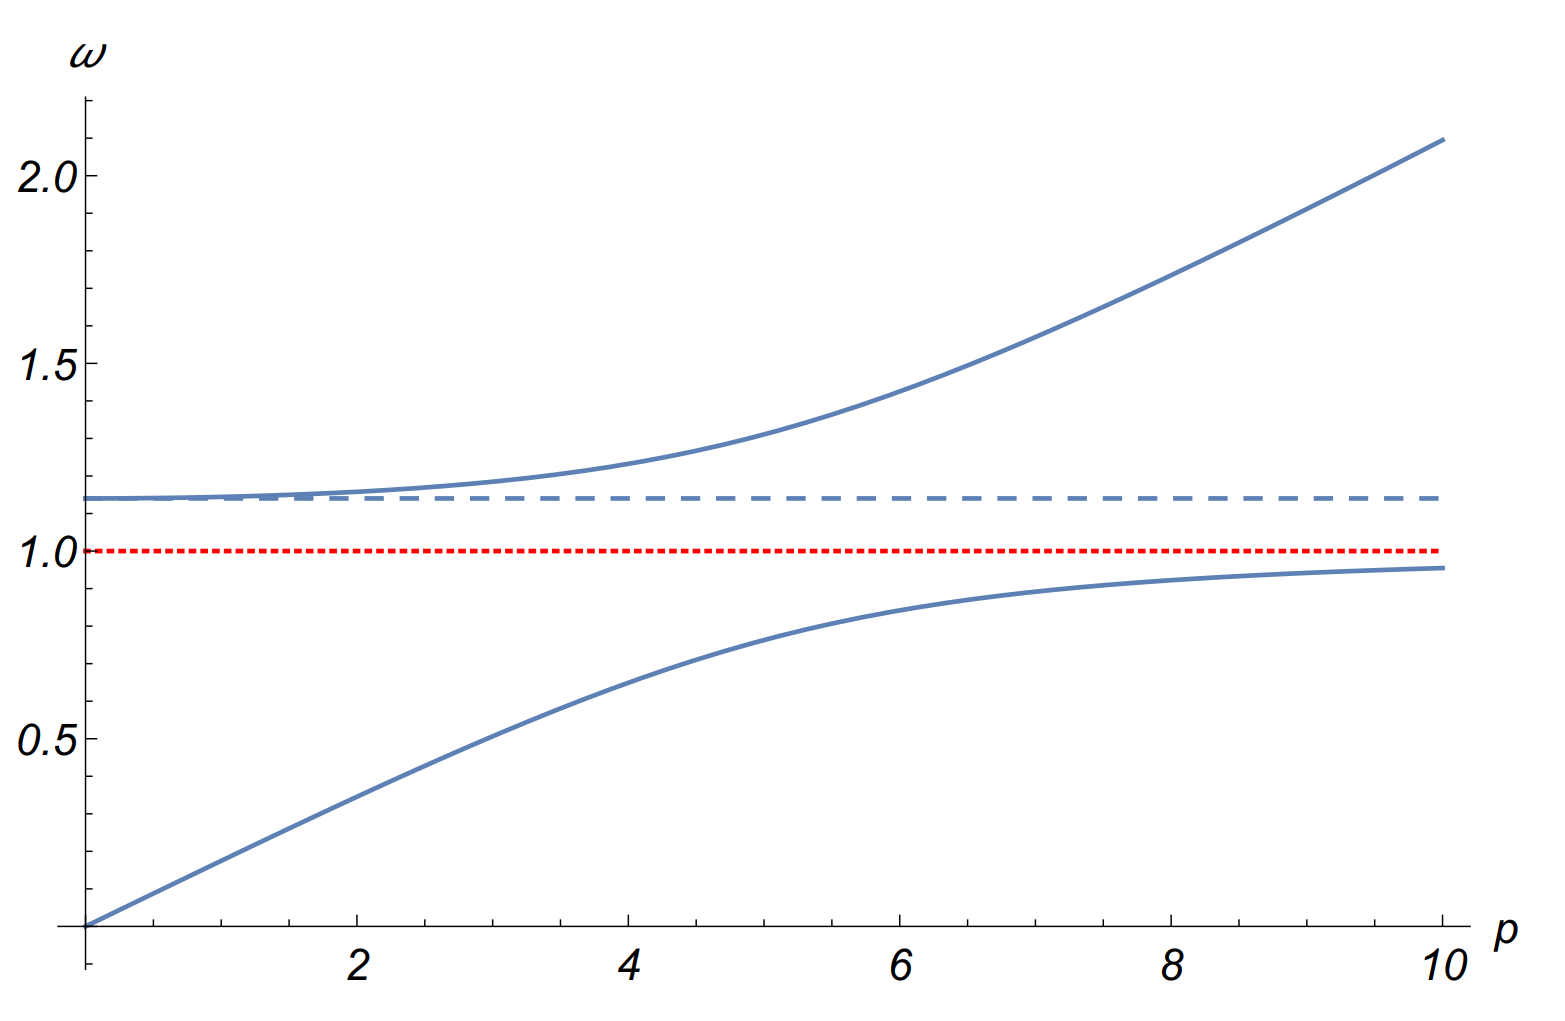
\includegraphics[width=0.75\textwidth]{disp_rel.png}
		\end{center}
		Акустическая и оптическая ветви колебаний, наличие запрещенной зоны, $\beta_0 = 1, \beta_1 = 1, h = 0.2, \eta = 0.3$.
	\end{figure}
\end{frame}



\subsection{Генерация и управление гармоническими волнами}

\begin{frame}
	\frametitle{Генерация волн}
	Начальные и граничные условия для численного решения с целью генерации бегущих волн,
	$$
	u(0,t)=\frac{\beta_1-\omega^2}{\beta_1}~B~ {\text{sin}} (\omega ~t),~u(x,0)=0, ~u(x,0)_t=0,
	$$
	$$
	v(0,t)=B ~{\text{sin}} (\omega ~t),~v(x,0)=0, ~v(x,0)_t=0.
	$$
	На правой границе --- условие поглощения. Реализуется с использованием подхода маскирующего потенциала, система переписывается в виде
	$$
	U_{t}=\beta_0 h^2 u_{xx}+\eta \beta_1 (v-u)
	$$
	$$
	u_{t}=U + u f_{\text{mask}},
	$$
	$$
	v_{tt}=-\beta_1 (v-u),
	$$
	где $ f_{\text {mask}} = \log \left[ \left(\tanh {0.03 (3 x_N - x)} \right)^2 \right] $, при интервале интереса от $0$ до $x_N$ и расчетном интервале от $0$ до $3 x_N$.
\end{frame}

\begin{frame}
	\begin{small}
	$t_N = 600; x_N = 60;\beta_0=1, h = 0.5, \beta_1 = 0.1, \eta = 0.5,  B=0.25$, запрещенная зона $0.316<\omega<0.387$.
	\end{small}
	\begin{figure}
		\begin{center}
			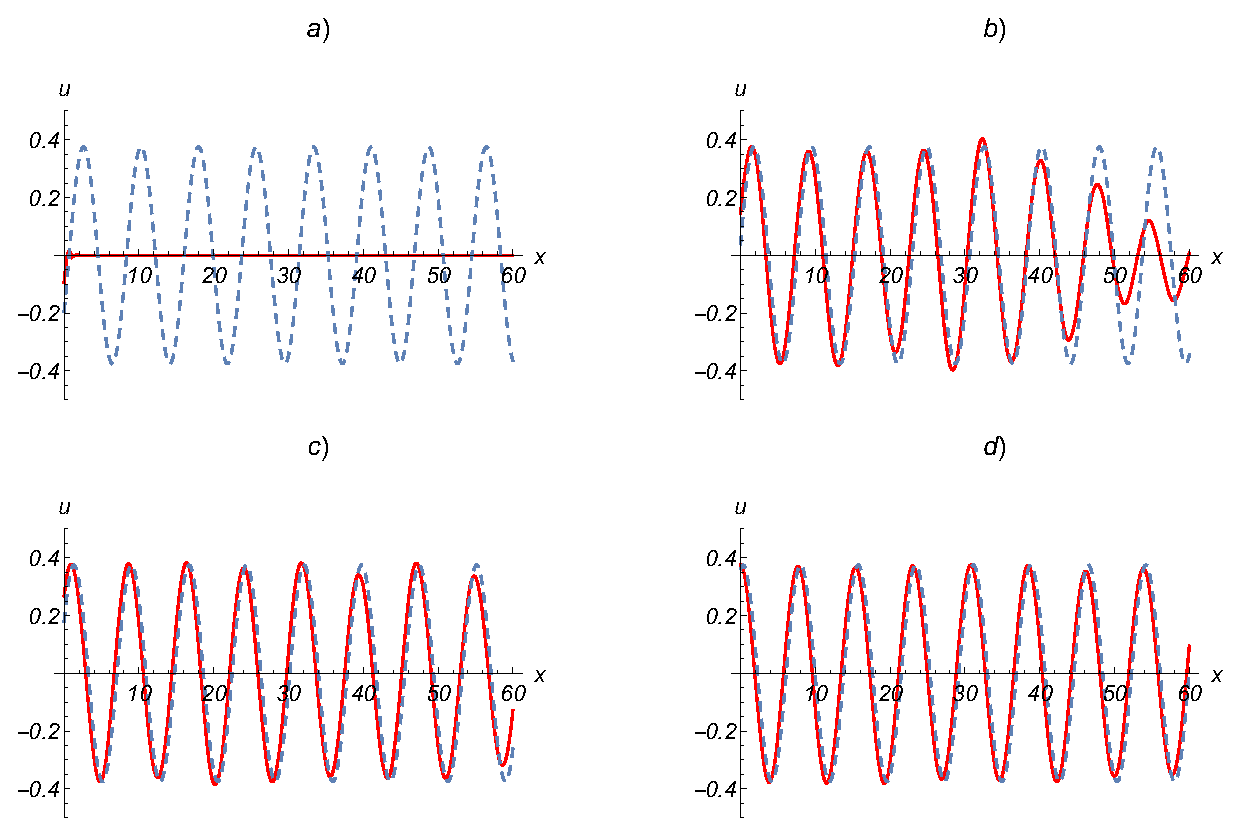
\includegraphics[width=0.9\textwidth]{new_pic/fig1.eps}
		\end{center}
		Генерация бегущей волны $u$ ниже запрещенной зоны в разные моменты времени, $\omega = 0.2 < \sqrt{\beta_1}$.  a) $t=0$; b) $ t=t_N/4$; c) $t=t_N/2$; d) $t=t_N$.
	\end{figure}
\end{frame}

\begin{frame}
	\begin{small}
		$t_N = 600; x_N = 60;\beta_0=1, h = 0.5, \beta_1 = 0.1, \eta = 0.5,  B=0.25$, запрещенная зона $0.316<\omega<0.387$.
	\end{small}
	\begin{figure}
		\begin{center}
			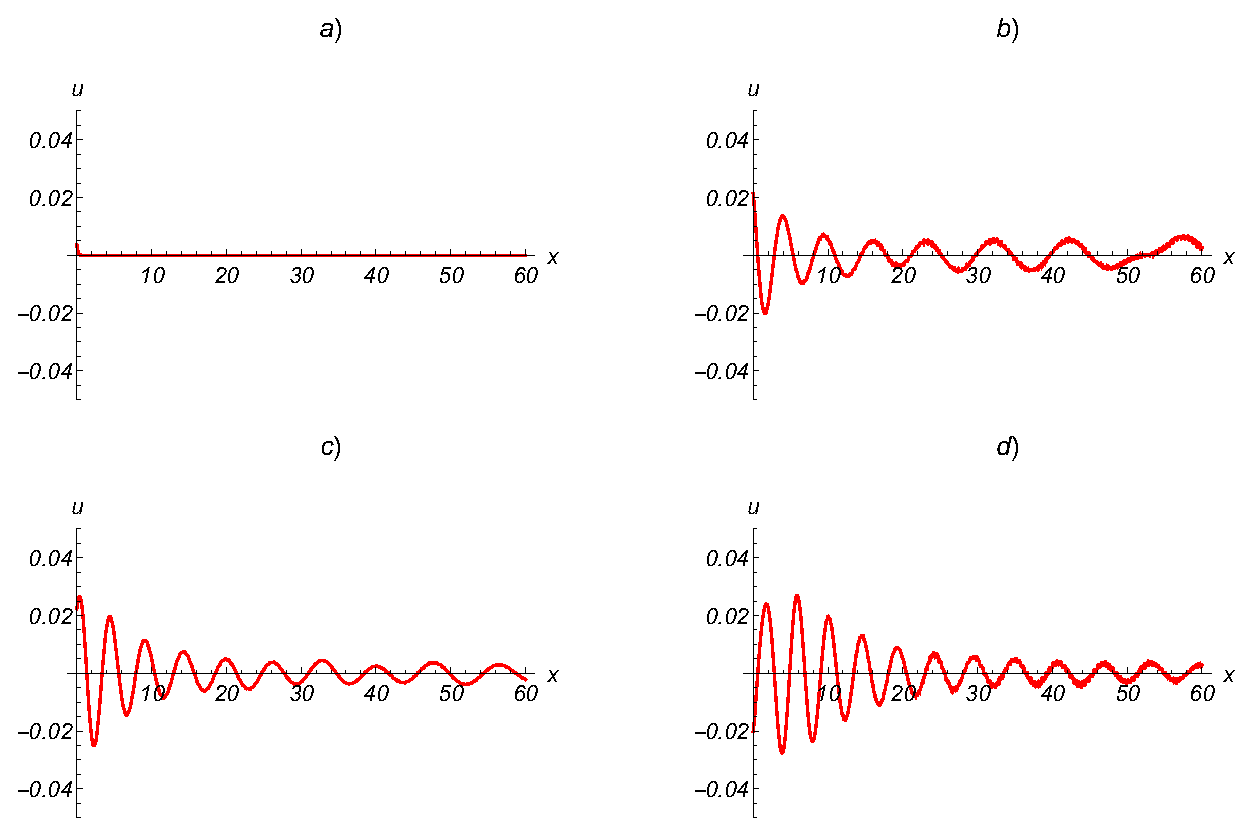
\includegraphics[width=0.9\textwidth]{new_pic/fig2.eps}
		\end{center}
		Генерация бегущей волны $u$ на нижней границе запрещенной зоны в разные моменты времени, $\omega = 0.3 \approx \sqrt{\beta_1}$.  a) $t=0$; b) $ t=t_N/4$; c) $t=t_N/2$; d) $t=t_N$.
	\end{figure}
\end{frame}

\begin{frame}
	\begin{small}
		$t_N = 600; x_N = 60;\beta_0=1, h = 0.5, \beta_1 = 0.1, \eta = 0.5,  B=0.25$, запрещенная зона $0.316<\omega<0.387$.
	\end{small}
	\begin{figure}
		\begin{center}
			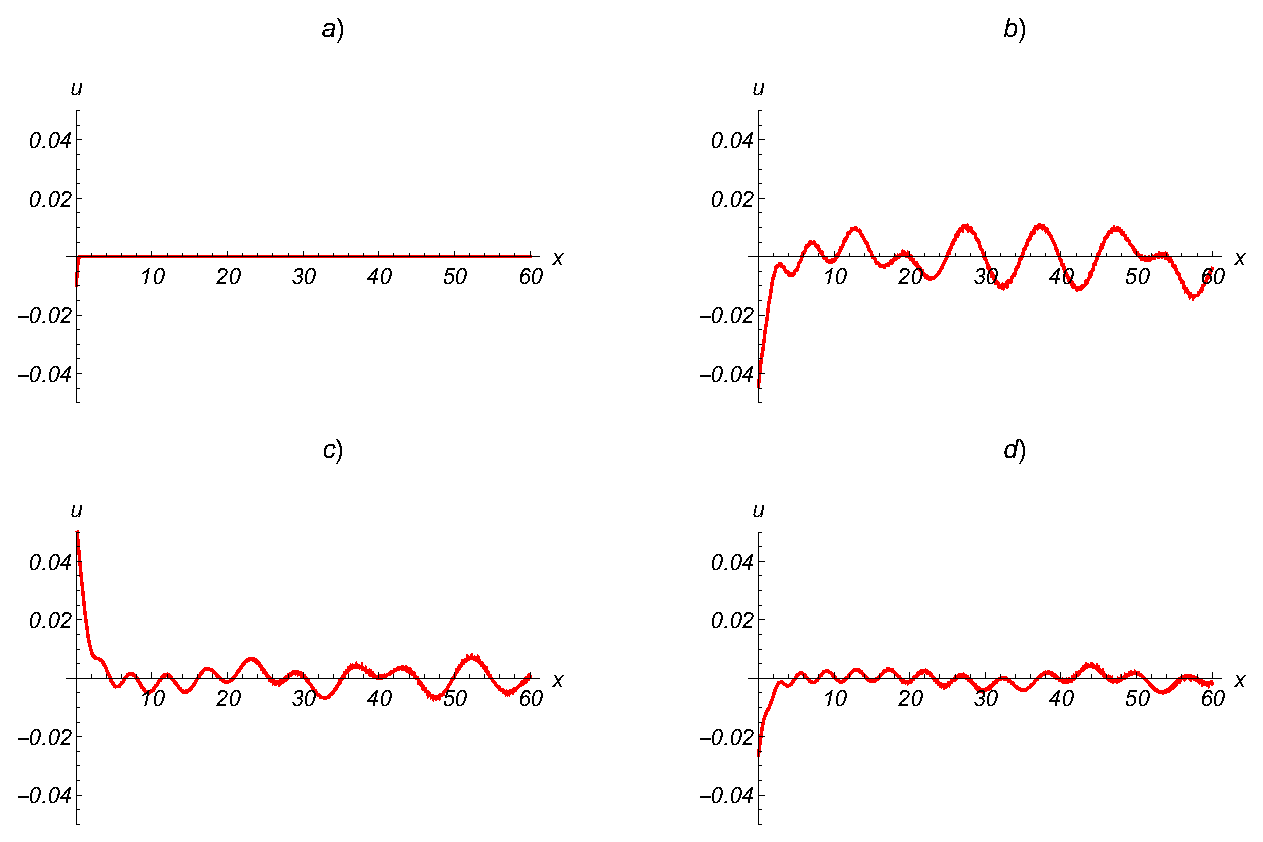
\includegraphics[width=0.9\textwidth]{new_pic/fig3.eps}
		\end{center}
		Генерация бегущей волны $u$ внутри запрещенной зоны в разные моменты времени, $\omega = 0.35 < \sqrt{\beta_1}$.  a) $t=0$; b) $ t=t_N/4$; c) $t=t_N/2$; d) $t=t_N$.
	\end{figure}
\end{frame}

\begin{frame}
	\frametitle{Управление включением}
	Управление волнами может быть реализовано использованием электромагнитных сигналов в для изменения внутренних свойств метаматериала, рассматривается механизм мгновенного включения,
	$$
	u_{tt}=\beta_0 h^2 u_{xx}+\eta \beta_1 (v-u)~H(t_0-t)
	$$
	$$
	v_{tt}=-\beta_1 (v-u) ~H(t_0-t)
	$$
	Включение управления предполагает переход уравнений движений к режиму волнового уравнения, решение которого будет иметь вид
	$$
	u_w=\frac{\beta_1-\omega^2}{\beta_1}~B~{\text{sin}}  (\imath(\omega/a~ x - \omega~ t-\omega/a~ x_0))
	$$
\end{frame}

\begin{frame}
	\begin{figure}
		\begin{center}
			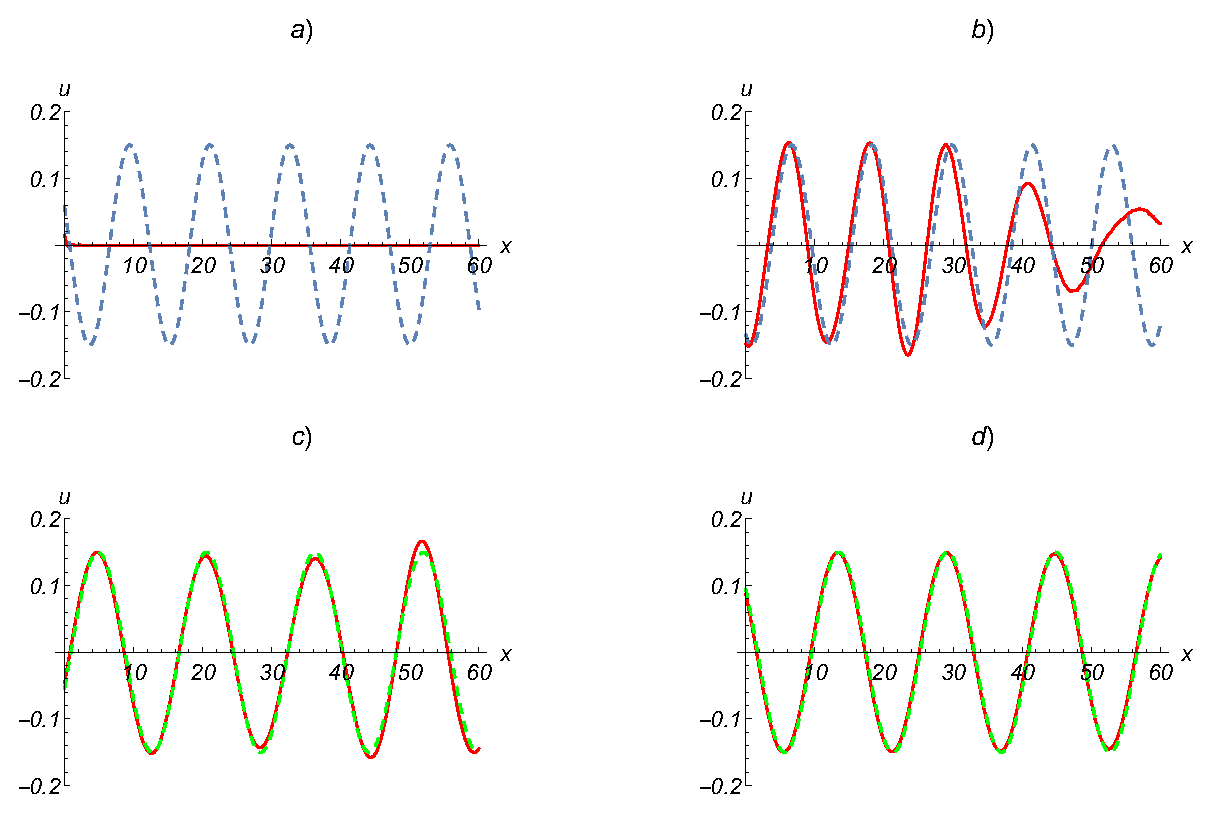
\includegraphics[width=0.9\textwidth]{new_pic/fig4.eps}
		\end{center}
		Управление включением, частота ниже запрещенной зоны в разные моменты времени, $\omega = 0.2$.  a) $t=0$; b) $ t=t_0=t_N/4$; c) $t=t_N/2$; d) $t=t_N$.
	\end{figure}
\end{frame}

\begin{frame}
	\begin{figure}
		\begin{center}
			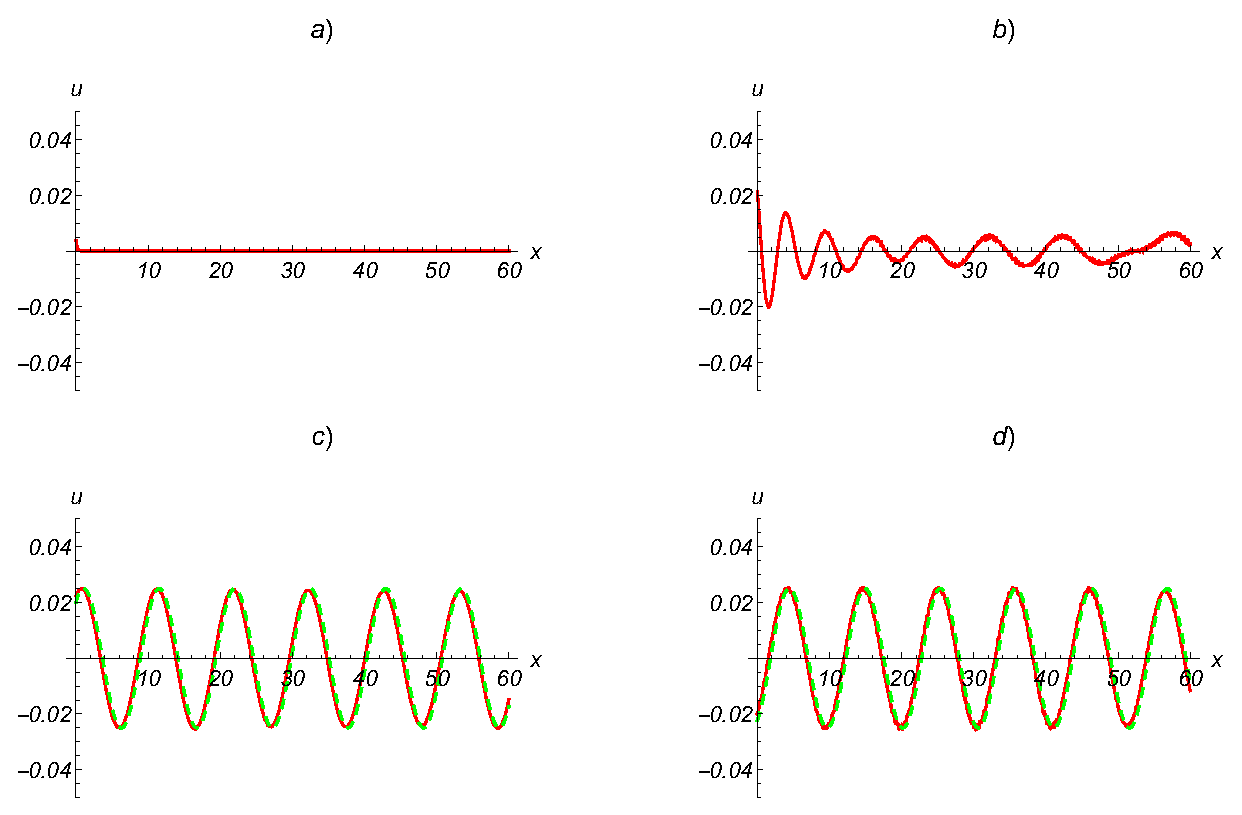
\includegraphics[width=0.9\textwidth]{new_pic/fig5.eps}
		\end{center}
		Управление включением, частота на нижней границе запрещенной зоны в разные моменты времени, $\omega = 0.3$.  a) $t=0$; b) $ t=t_0=t_N/4$; c) $t=t_N/2$; d) $t=t_N$.
	\end{figure}
\end{frame}

\begin{frame}
	\begin{figure}
		\begin{center}
			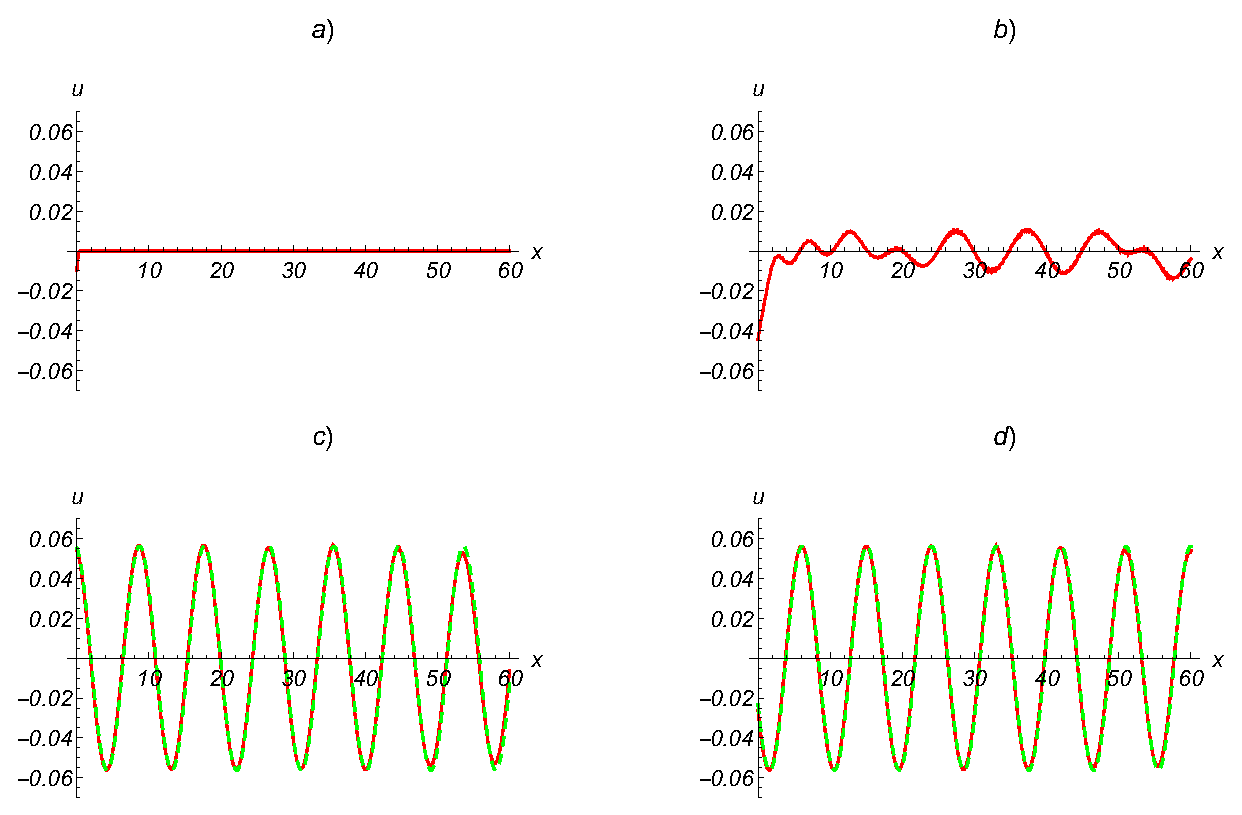
\includegraphics[width=0.9\textwidth]{new_pic/fig6.eps}
		\end{center}
		Управление включением, частота внутри запрещенной зоны в разные моменты времени, $\omega = 0.35$.  a) $t=0$; b) $ t=t_0=t_N/4$; c) $t=t_N/2$; d) $t=t_N$.
	\end{figure}
\end{frame}

\subsection{Основные результаты}
\begin{frame}
	\frametitle{Результаты}
	Основные результаты данной части работы заключаются в следующем,
	\begin{itemize}
		\item{Граничное возбуждение может генерировать гармонические волны в метаматериале, что согласуется с результатами, полученными на основе конкретного решения в виде бегущей волны;}
		\item{Численно продемонстрировано, как управление включением позволяет менять режим распространения волн;}
		\item{Дальнейшие перспективы могут быть связаны с рассмотрением модели активного метаматериала под действием внешней силы, обеспечивающей управление обратной связью, а также обобщение модели на нелинейный случай.}
	\end{itemize}
\end{frame}

\section{Численные методы исследования волновых процессов в двумерных решетках}
\subsection{Постановка задачи}
\subsection{Численный метод}
\subsection{Основные результаты}

\begin{frame} % публикации на одной странице
	% \begin{frame}[t,allowframebreaks] % публикации на нескольких страницах
	\frametitle{Публикации по теме диссертации}
	\begin{small}
\begin{enumerate}
	\item \textit{Porubov, A. V.} Further progress in control of localized nonlinear waves [Текст] / A. V. Porubov, I. D. Antonov, A. L. Fradkov // Journal of Physics: Conference Series. -- 2017. -- Дек. -- Т. 937. -- С. 012043.	
	
	\item \textit{Porubov, A. V.} Nonlinear Dynamics of Two-Dimensional Lattices with Complex Structure [Текст] / A. V. Porubov, A. E. Osokina, I. D. Antonov // Advanced Structured Materials. -- Springer International Publishing, 2020. -- С. 309--334.
	
	\item \textit{Porubov, A. V.} Boundary control of nonlinear strain waves in di-atomic crystal layer [Текст] / A. V. Porubov, I. D. Antonov, A. L. Fradkov // Wave Motion. -- 2019. -- Нояб. -- Т. 91. -- С. 102400.
	
	\item \textit{Porubov, A. V.} On control of harmonic waves in an acoustic metamaterial [Текст] / A. V. Porubov, I. D. Antonov // Mechanics Research Communications. -- 2021. -- Сент. -- Т. 116. -- С. 103745.
	
	\item \textit{Антонов, И. Д.} Управление нелинейными локализованными волнами в механических системах [Текст] / И. Д. Антонов, А. В. Порубов // Нелинейные волны, XVIII научная школа, Нижний Новгород. -- 2018
\end{enumerate}
\end{small}
\end{frame}


\begin{frame}
\frametitle{Другие публикации}
\begin{tiny}
\begin{enumerate}
	\item \textit{Antonov, I. D.} Pseudo-three-dimensional model for hydraulic fracturing with foams [Текст] / I. D. Antonov // Journal of Physics: Conference Series. -- 2019. -- Июнь. -- Т. 1236. -- С. 012055. -- URL: https://doi.org/10.1088/1742-6596/1236/1/012055.
	
	\item \textit{Antonov, I. D.} Numerical modeling of hydraulic fracturing with foams and energized fluids [Текст] / I. D. Antonov // 28TH RUSSIAN CONFERENCE ON MATHEMATICAL MODELLING IN NATURAL SCIENCES. -- AIP Publishing, 2020. -- URL: https://doi.org/10.1063/5.0004658.
	
	\item \textit{Antonov, I. D.} Two-dimensional model for hydraulic fracturing with foams [Текст] / I. D. Antonov, A. V. Porubov, N. M. Bessonov // Material Physics and Mechanics. -- 2018. -- Т. 40.1. -- URL: https://mpm.spbstu.ru/article/2018.65.5/.
	
	\item \textit{Porubov, A. V.} Influence of compressibility on the foam fracture modeling [Текст] / A. V. Porubov, I. D. Antonov // Journal of Physics: Conference Series. -- 2019. -- Апр. -- Т. 1205. -- С. 012048. -- URL: https://doi.org/10.1088/1742-6596/1205/1/012048.
	
	\item Strain localization in two-dimensional lattices [Текст] / A. V. Porubov, I. Antonov, A. Sokolov, W. H. Muller // Journal of Physics: Conference Series. -- 2020. -- Дек. -- Т. 1686. -- С. 012036. -- URL: https://doi.org/10.1088/1742-6596/1686/1/012036.
	
	\item Geometrically nonlinear dynamic model for a hexagonal lattice [Текст] / A. V. Porubov, A. M. Krivtsov, I. Antonov, W. H. Muller, A. A. Sokolov // Physical Review E. -- 2020. -- Авг. -- Т. 102, № 2. -- URL: https://doi.org/10.1103/physreve.102.022209.
	
	\item Mechanical system allowing distributive control with feedback [Текст] / A. V. Porubov, I. D. Antonov, D. A. Indeitsev, A. L. Fradkov // Mechanics Research Communications. -- 2018. -- Окт. -- Т. 93. -- С. 124--127. -- URL: https://doi.org/10.1016/j.mechrescom.2017.07.014.
	
	\item Control of localized non-linear strain waves in complex crystalline lattices [Текст] / A. V. Porubov, I. D. Antonov, A. L. Fradkov, B. R. Andrievsky // International Journal of Non-Linear Mechanics. -- 2016. -- Нояб. -- Т. 86. -- С. 174--184. -- URL: https://doi.org/10.1016/j.ijnonlinmec.2016.09.002.
	
	\item \textit{Porubov, A. V.} Control of coupled localized nonlinear wave solutions [Текст] / A. V. Porubov, I. D. Antonov // Journal of Physics: Conference Series. -- 2017. -- Янв. -- Т. 788. -- С. 012029. -- URL: https://doi.org/10.1088/1742-6596/788/1/012029.
	
\end{enumerate}
\end{tiny}
\end{frame}

\begin{frame}[plain, noframenumbering] % последний слайд без оформления
	\begin{center}
		\Huge
		Спасибо за внимание!
	\end{center}
\end{frame}

